\section{Experiment 3: EVS Resampling Study}

In the third experiment, we performed a resampling study based on the EVS data to assess the 
how the result obtained for Experiments 1 and 2 carry over to real data applications.
EVS is a large-scale, cross-national survey on human values administered in almost 50 countries
across Europe.
It covers a wide range of human values regarding family, work, environment, perceptions of 
life, politics and society, religion and morality, national identity.
It is a high-quality survey widely used for comparative studies between European countries.
Furthermore, it is accessible free of charge and it represents the type of data social scientist 
regularly analyse.
Variables in the EVS data are discrete numerical and categorical items following a 
variety of distributions.
By using data gathered for an actual survey, we could study whether the relative performances of 
the imputation methods, displayed in the simulation studies, changed when deployed for real data 
research.

\subsection{Resampling Study Procedure} \label{resProc}

\subsubsection{Data preparation and generation}
	For this study, we used the third pre-release of the 2017 wave of EVS data \citep{EVS:2017} to define
	a population dataset with no missing values.
	The original dataset contained 55,000 observations from 34 countries.
	We selected only the four founding countries of the European Union included in the dataset (France, Germany,
	Italy, and the Netherlands) and excluded all columns of the data that were either duplicated
	information (recoded versions of other variables), or meta data (e.g. time of interview,
	mode of data collection). 
	All originally missing values were filled in with a run of a single imputation predictive mean matching (PMM) 
	algorithm to obtain a pseudo fully-observed dataset.
	This imputation step was completed by using the $mice$ R package imputation procedure.
	PMM was chosen for the task as it is a flexible imputation method that maintains the distributional 
	characteristics of the original data.
	Predictors for the imputation models were selected based on the variable selection procedure described in
	\citeauthor{vanBuurenEtAl:1999} (\citeyear[pp. 687–688]{vanBuurenEtAl:1999}) by using the \emph{quickpred()}
	R function and setting the minimum correlation threshold to 0.3.
	The number of iterations was set to 200.
	This imputation procedure is used to obtain a pseudo-population dataset, and therefore it does not require
	multiple imputation itself.

	At the end of this data cleaning process, we obtained a fully-observed dataset ($\bm{Z}$) of 8,045 observations 
	($n$), across 4 countries, and 243 variables ($p$).
	For every repetition of the first step in the resampling procedure, a bootstrap sample $\bm{Z}^{*}$ was 
	generated by sampling with replacement $n$ observations from the EVS population data $\bm{Z}$.
	We considered two conditions in the resampling study: low and high dimensional data.
	As the number of predictors in the data was fixed ($p = 243$), the dimensionality of the data was 
	changed by defining different sizes for the sample taken from the pseudo-fully observed data in
	step 1.
	We chose two values for $n$, namely $1,000$ and $300$, corresponding to a low and high 
	dimensional condition.

\subsubsection{Analysis models}

	To define plausible analysis models, we searched for models that have been used in published articles
	testing social scientific theories on the EVS data.
	The search was performed by screening the repository of publications using EVS data available on the EVS 
	website \citep{EVSbib}.

	As a result, we defined two linear regression models, models 1 and 2, of the same form:
%	
	\begin{equation}
		y = \beta_{0} + \beta_{1} x + \bm{\beta} \bm{C}  \label{eqn:lm}
	\end{equation}
%
	where a dependent variable $y$ is regressed on a variable of interest $x$ and a set of control variables
	$\bm{C}$.
	In this scenario, $\beta_{1}$ is a focal parameter that a researcher wants to use to test some hypothesis.

	The first version of linear model \eqref{eqn:lm}, Model 1, was inspired by \cite{koneke:2014}:
	$y^{(1)}$, its dependent variable, was a 10-point EVS item measuring euthanasia acceptance 
	(`Can [euthanasia] always be justified, never be justified, or something in between?');
	the predictor of interest $x^{(1)}$ was a 4-point item measuring the self-reported importance of religion in 
	one's life;
	the matrix of covariates $\bm{C}^{(1)}$ included trust in the health care system, trust in the state, 
	trust in the press, country, sex, age, education, and religious denomination.
	This model represents a plausible analysis a researcher would perform to test a hypothesis regarding the 
	effect of religiosity on the acceptance of end-of-life treatments.

	Model 2, the second version of the linear model in equation \ref{eqn:lm}, was inspired by \cite{immerzeel:2015}.
	The dependent variable $y^{(2)}$ was an harmonized variable constructed by EVS to describe the respondents' 
	tendency to vote left or right-wing parties, expressed on a 10-point left-to-right continuum.
	The predictor of interest $x^{(2)}$ was a scale measuring respondents' attitudes toward immigrants and immigration 
	(`nativist attitudes scale').
	The scale was obtained by taking the average of respondents' agreement, on a scale from 1 to 10, with three 
	statements: `immigrants take jobs away from natives', `immigrants increase crime problems', and 
	`immigrants are a strain on welfare system'.
	The control variables used were: 
	attitudes toward law and order, attitudes toward authoritarianism, interest in politics, level of political activity,  
	country, sex, age, education, employment status, socio-economic status, importance of religion in life, 
	religious denomination, and the size of town where interview was conducted.
	A researcher might fit this model and look at the value and standard error of $\beta^{(2)}_{1}$, 
	the `nativist attitude' regression coefficient, to test an hypothesis regarding the effect of xenophobia on voting 
	tendencies.

\subsubsection{Missing data imposition}

	Missing data were imposed on 6 variables according to the same strategy described in Subsection \ref{sub_missing}.
	The variables target of missing value imposition were the euthanasia acceptance item $y^{(1)}$, and the 
	left-to-right voting tendency $y^{(2)}$, the two dependent variables in models 1 and 2; 
	religiosity ($x^{(1)}$, focal and control variable in models 1 and 2 respectively), 
	and the three items making up the ``nativist attitudes'' scale (focal predictor $x^{(2)}$
	in the second model).

	The response model form was the same as in Equation \eqref{eqn:rm} and three variables were included in $\tilde{Z}$: 
	age, education, and an item measuring trust in new people. 
	Older people tend to have higher item non-response rates than younger people, and 
	lower educated people tend to have higher item non-response rates than higher educated people 
	\citep{guadagnoliCleary:1992, leeuwEtAl:2003}.
	We assumed that people with less trust in strangers have a higher item non-response tendency as 
	they are likely to withhold more information from the interviewer (a stranger).

\subsubsection{Imputation}
	
	Missing values were treated according to all the methods described in Section 2.
	The imputation methods were parametrized as in Experiments 1 and 2.
	Here, we describe the key details in the algorithms specifications.

	\paragraph{Convergence}

	As for the simulation studies, convergence of the imputations was assessed in a pre-processing step.
	Before running the actual resampling study, 10 datasets were sampled from the EVS populaton data and missing 
	values were imposed.
	Missing values were then imputed by running 5 parallel imputation chains for each Multiple Imputation 
	method.
	Convergence was checked by observing mean imputations trace-plots.
	This procedure was performed only for condition 2, the high-dimensional one, under the assumption that convergence
	would be faster in the low-dimensional set up.
	After the convergence check, we decided to run the algorithms for the regular experiment run for 60 iterations 
	before saving the multiply imputed datasets, although most methods achieved convergence well before that number 
	of iterations.

\subsection{Results}

	\subsubsection{Single Parameter of interest}

	Figures \ref{fig:exp4bias} and \ref{fig:exp4ci} report the PRB and the CIC for parameters $\beta^{(1)}_{1}$ and 
	$\beta^{(2)}_{1}$, the focal regression coefficients in the two models.
	Most of the MI methods resulted in negligible biases ($|PRB| < 10\%$) for both parameters in all conditions.
	The only two exceptions were bridge and MI-RF. 
	The former was very competitive in the low-dimensional condition, but led to extreme bias and 
	over-coverage in the high-dimensional condition for $\beta_{1}$ in Model 1; 
	the latter provided the largest PRBs and worst CIs (under) coverage for the focal regression coefficients among 
	the other MI methods, and it was consistently outperformed even by Complete Case analysis.
	missForest also displayed contained focal parameter biases.
	DURR and IURR gave inconsequential biases for both parameters in all conditions, with PRBs that were
	often at least half in size as the ones obtained with the other methods, outperforming even MI-OP in the high 
	dimensional condition for $\beta_{1}$ in Model 2.
	For $\beta_{1}$ in Model 2, both IURR and DURR remained fairly competitive in terms of coverage 
	with CICs close to nominal levels, but the advantage they showed in terms of bias was not carried over to 
	this criterion.
	Both MI-PCA and Blasso provided CICs either equal or closer to nominal than the ones obtained with
	IURR and DURR in almost all conditions.

	As for $\beta^{(1)}$ in Model 1, all MI methods led to under-coverage of the true parameter values with CIC smaller 
	than the threshold value 0.94.
	Although coverage of the true values was not particularly good for any of the methods selected, the Gold Standard
	confidence intervals were also under-covering the true value of $\beta_{1}$ in Model 1.
	This was likely due to the right-skewed nature of the distribution of the dependent variable (euthanasia 
	acceptance).
	Most MI imputation methods achieved coverages similar to that of the Gold Standard method, and more importantly 
	their relative difference, compared to the GS coverages, was in line with what can be seen for $\beta_{1}$ in Model 2.

\begin{figure}[h]
	\centering
	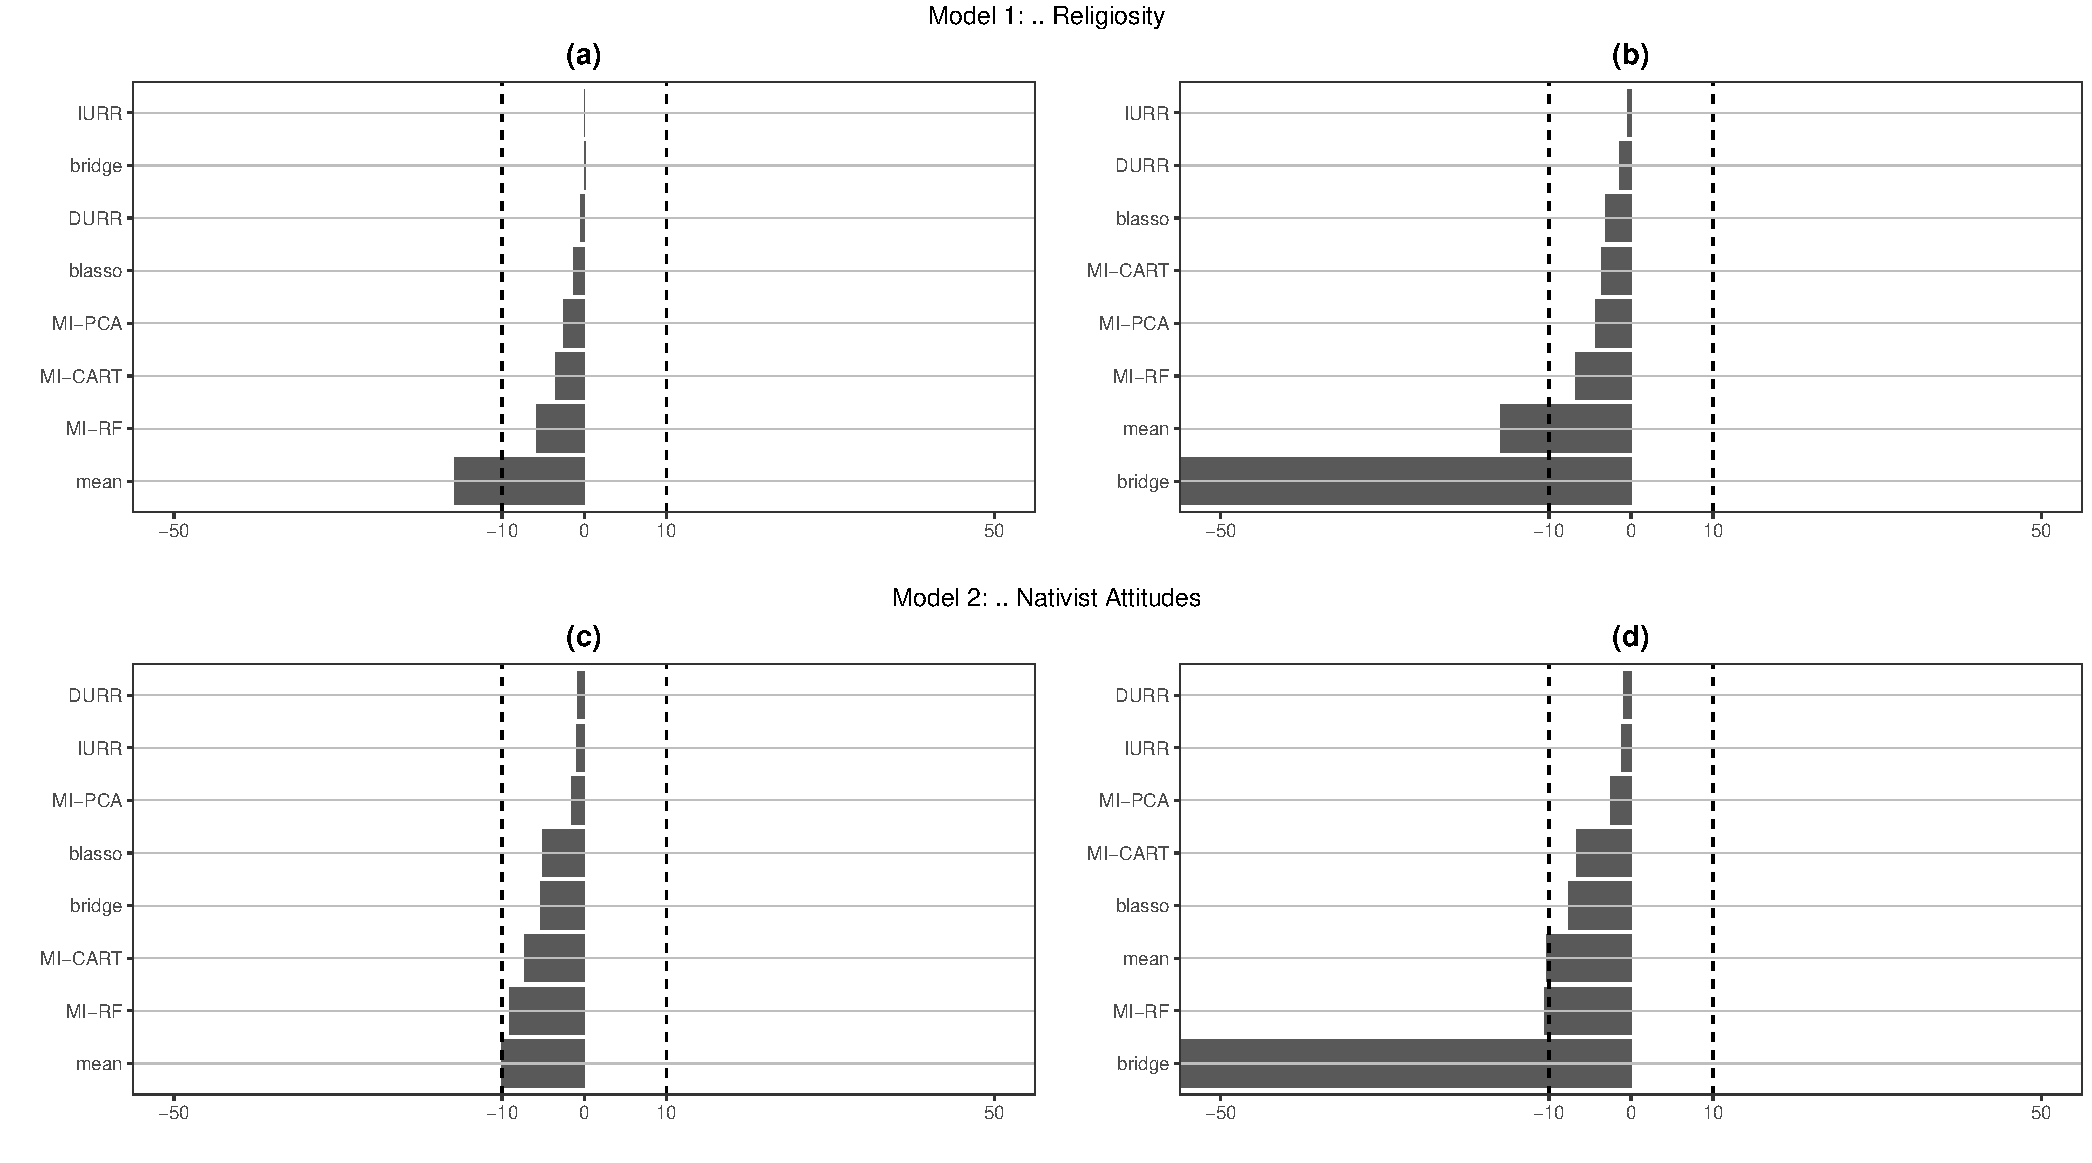
\includegraphics{\pathFIG/exp4_imp_bias.pdf}
	\caption{PRB in the estimation of parameters of interest $\beta^{(1)}_{1}$ and $\beta^{(2)}_{1}$, 
		in model 1 and 2 respectively}
	\label{fig:exp4bias}
\end{figure}

\begin{figure}[h]
	\centering
	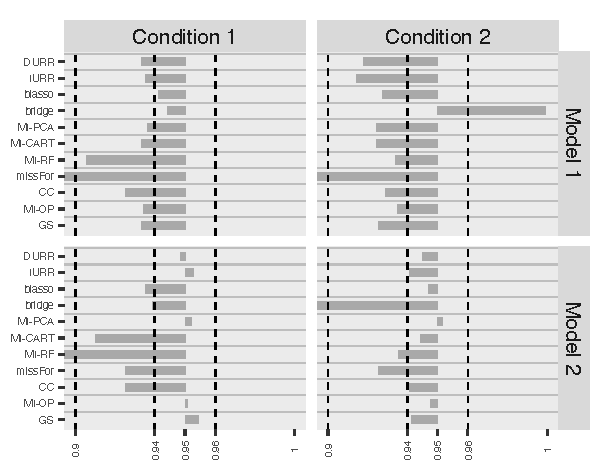
\includegraphics{\pathFIG/exp4_imp_ci.pdf}
	\caption{CIC in the estimation of parameters of interest $\beta^{(1)}_{1}$ and $\beta^{(2)}_{1}$, 
		in model 1 and 2 respectively}
	\label{fig:exp4ci}
\end{figure}

\FloatBarrier

	\subsubsection{Overall Model Parameter Assessment}
	The estimated linear models were multiple regressions, and all regression coefficient estimates were 
	influenced by the imputations.
	Therefore, it is important to observe the overall effects of the different methods on model estimation.
	Figure \ref{fig:exp4_bias_allP} reports the absolute values of the PRBs for every Model 2 parameter 
	estimate, ordered by size, under each of the different imputation methods.
	(see figures \ref{fig:exp4bias_m1} and \ref{fig:exp4cir_m1} in the Appendix for Model 1 results).
	MI-OP showed that even having perfect information regarding the missing data mechanism and data structure,
	results in some bias for certain estimates.
	Although the bias for the intercept and the focal parameter were negligible, around half of the estimates 
	obtained after using this imputation method showed large biases ($|PRB|>10\%$), and the largest bias was 
	considerable (around 40\%, in the low dimensional condition, and 20\%, in the high-dimensional one).
	In both the high- and low-dimensional conditions, MI using DURR, IURR, Blasso, and MI-CART, and SI using 
	missForest showed fairly similar overall patterns to MI-OP, with only slightly larger PRBs.
	MI-PCA and MI-RF showed similar trends but they presented overall larger PRBs for those estimates 
	exceeding the 10\% threshold.
	However, none of these methods seemed to suffer from the increase in dimensionality.
	Bridge demonstrated the same results described in the simulation studies. 
	It was a competitive method in low dimensional scenarios, but it was inadequate to deal with high-dimensional 
	data imputation (all but one PRB are larger than 100\%).

	Figure \ref{fig:exp4_ci_allP} reports the CIC for each parameter estimate in model 2.
	When using MI-OP, CICs showed a deviation from nominal coverage for only two parameters, with a slight 
	tendency toward over-coverage.
	While DURR, IURR, MI-CART and MI-PCA maintained a similar coverage pattern to MI-OP, 
	blasso, MI-RANF, and missforest were either over- or under-covering many more parameters.
	The results showed by missForest were as expected. 
	A single imputation approach, it underestimates uncertainty regarding values of the empty data cells, 
	and tends to produce narrower confidence intervals.
	Despite showing poor performances in terms of bias, Complete Case analysis manifested good 
	coverage.
	However, this was a result of the smaller sample size used for estimating the analysis model, rather than 
	a positive feature of the method.
	The smaller samples produced wider intervals which covered the true values even when the point-estimates 
	were biased.

\begin{figure}
	\centering
	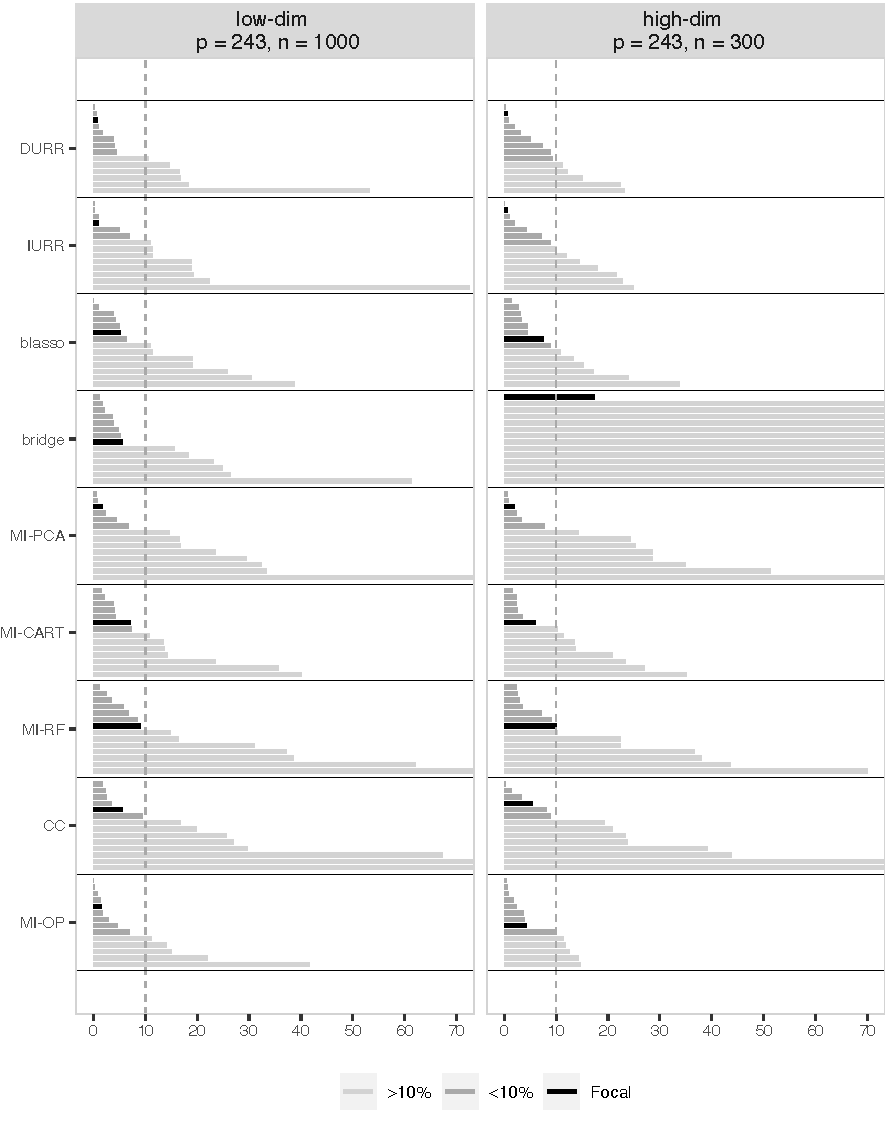
\includegraphics{\pathFIG/exp4_imp_bias_allParms_m2.pdf}
	\caption{PRBs for all the model parameters in model 2. 
		The order of the bars is based on the absolute value of the PRBs.
		The values for the intercept, the focal regression coefficient, and the regression coefficient with which most 
		methods struggle (Largest Bias) are highlighted}
	\label{fig:exp4_bias_allP}
\end{figure}

\begin{figure}
	\centering
	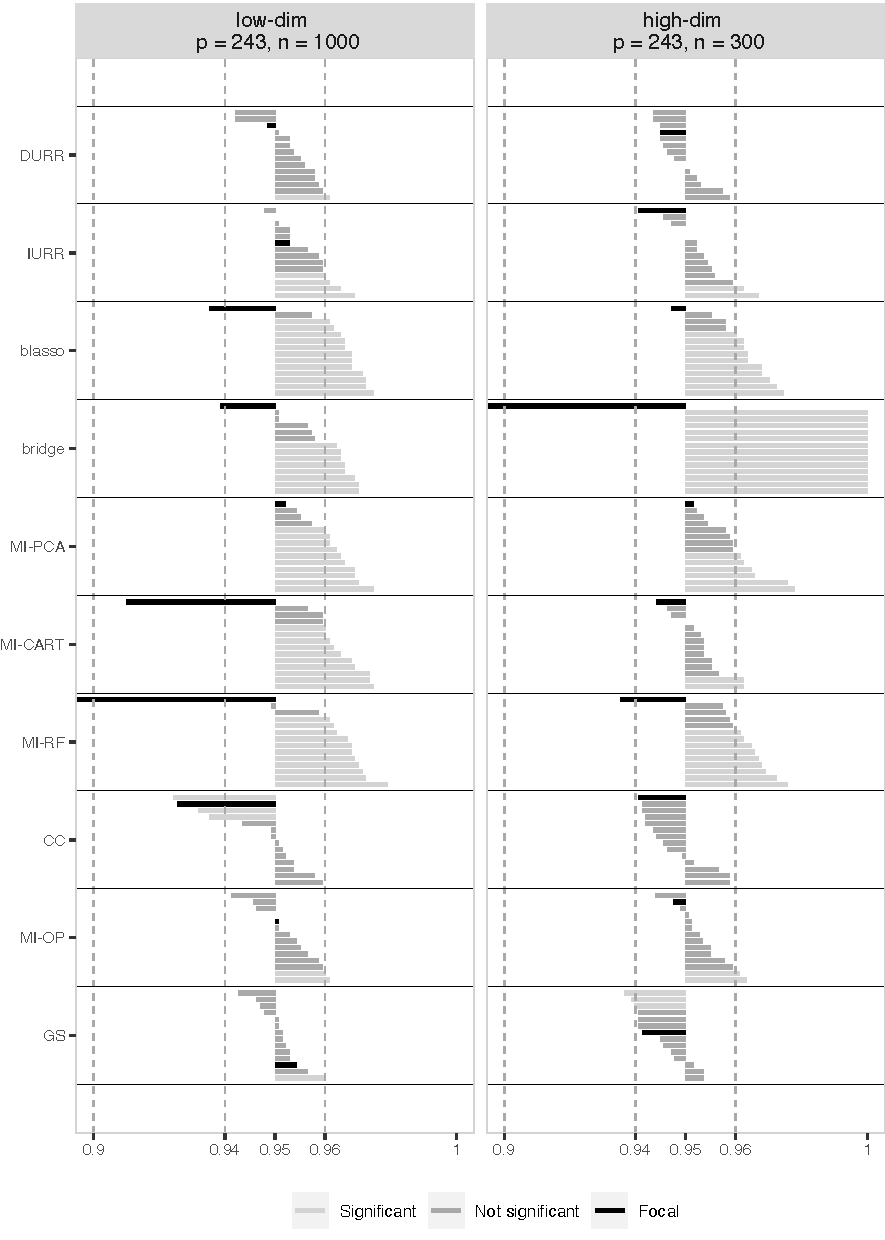
\includegraphics{\pathFIG/exp4_imp_ci_allParms_m2.pdf}
	\caption{CIC for all model parameter in model 2.
		Bars are sorted in by ascending value.
		The values for the intercept, the focal regression coefficient, and the regression coefficient with which most 
		methods struggle (Largest Bias) are highlighted}
	\label{fig:exp4_ci_allP}
\end{figure}

\FloatBarrier

\subsubsection{Imputation Time}

	Table \ref{tab:time} reports the average imputation time for the different methods.
	IURR and DURR were the most time-consuming methods with imputation times above the hour 
	in our low-dimensional conditions. 
	MI-PCA and Blasso imputation had imputation times of a minute or less.
	In the high-dimensional condition, IURR and DURR were not as time-intensive due to the smaller
	sample size, but still required more than ten times the time of MI-PCA and blasso imputation.

\begin{table}
	\centering
	\begin{tabular}{l | r | r | r | r | r | r | r | r }
		condition & DURR & IURR & blasso & bridge & MI-PCA & MI-CART & MI-RF & MI-OP \\
		\hline
		1 & 73.20 & 75.90 & 1.40 & 8.10 & 0.60 & 4.00 & 11.30 & 2.20 \\ 
		2 & 6.10 & 9.70 & 0.50 & 3.20 & 0.40 & 1.40 & 4.70 & 1.90 	
	\end{tabular}
	\caption{\label{tab:time}Average imputation time in minutes.}
\end{table}

\FloatBarrier


